% Section content template for individual Educative lessons
% This file contains the actual content for a specific section
% Generated from Educative API section content

% Section: Detailed Design of Google Maps
% Section ID: 6026783136940032
% Section Slug: detailed-design-of-google-maps
% Generated: 2025-12-07T23:06:22.102041

In this lesson, we'll discuss our detailed design by answering the following questions:

\begin{enumerate}
\item
\protect\phantomsection\label{qPVuc2EQntMrcPuut5mM8}
How do user requests benefit from segments?
\item
\protect\phantomsection\label{lGuP5Gnpf1y0UUjrlj2Ez}
How do we improve the user experience by increasing the accuracy of ETAs?
\end{enumerate}

\subsection{Segment setup and request handling}\label{7yE8E_9SV1BEh0wRXH_Df}
\\
This section will describe how the segment data is stored in the database and how user requests are handled using the already stored data.\\
\strut \\
Starting with the storage schema, we discuss how the segments are added and hosted on the servers and also how the user requests are processed.

\subsubsection{Storage schema}\label{mIp9Ck897FnJuTH8HxpD_}
\\
We store the following information for each segment:
\\
\textbf{Key-value store}:

\begin{itemize}
\item
\protect\phantomsection\label{tq-iT4EIFUobRafnY8RR1}
The segment's \texttt{ID}.
\item
\protect\phantomsection\label{-00Jm48oN8sF72QbWVpSm}
The \texttt{serverID} on which the segment is hosted.
\item
\protect\phantomsection\label{fmOIJpz2mvFKE1IwCO8S_}
In reality, each segment is a polygon, so we store boundary \texttt{coordinates} (latitude/longitude), possibly as a list.
\item
\protect\phantomsection\label{GUmF65lsZERc1XO0tHd_j}
A list of segment IDs of the \texttt{neighbors} segments.
\end{itemize}
\\
\textbf{Graph database}

\begin{itemize}
\item
\protect\phantomsection\label{TOd57CYa3uamyaz8WZnTJ}
The road network inside the segment in the form of a \texttt{graph}.
\end{itemize}

\begin{figure}[htbp]
 \centering
 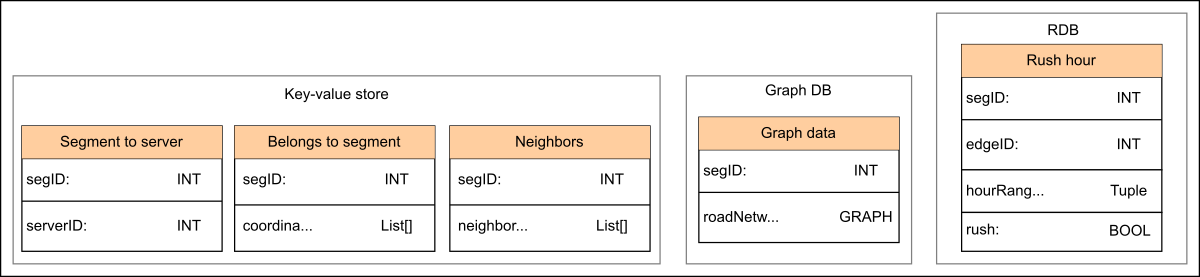
\includegraphics[width=0.5\textwidth]{Images/chapter_28/section_6026783136940032/5278741156855808.png}
 \caption{Storage schema}
\end{figure}

\textbf{Relational DB}
\\
We store the information to determine whether, at a particular hour of the day, the roads are congested. This later helps us decide whether or not to update the graph (weights) based on the live data.

\begin{itemize}
\item
\protect\phantomsection\label{623m6DzFlR8JDdv8WN84e}
\texttt{edgeID} identifies the edge.
\item
\protect\phantomsection\label{Vdehwz3gCzDtcr18XkuLj}
\texttt{hourRange} tells us which hour of the day it is when there are typical road conditions (non-rush hour) on the road.
\item
\protect\phantomsection\label{PmS-V7CzT27UEr5YuVBI-}
\texttt{rush} is a Boolean value that depicts whether there is congestion or not on a specific road at a specific time.
\end{itemize}
\begin{quote}
\textbf{Note:}\texttt{segID}, \texttt{serverID}, and \texttt{edgeID} are unique IDs generated by a uniqueID generator (see the \href{https://www.educative.io/courses/grokking-the-system-design-interview/system-design-sequencer}{Sequencer} lessons for details).
\end{quote}
\subsubsection{Design}\label{XAKO9jIpbD5sny_KXh0Gf}
\\
The following illustration consists of two workflows. One adds segments to the map and hosts them on the servers, while the other shows how the user\textquotesingle s request to find a path between two points is processed.

\begin{figure}[htbp]
 \centering
 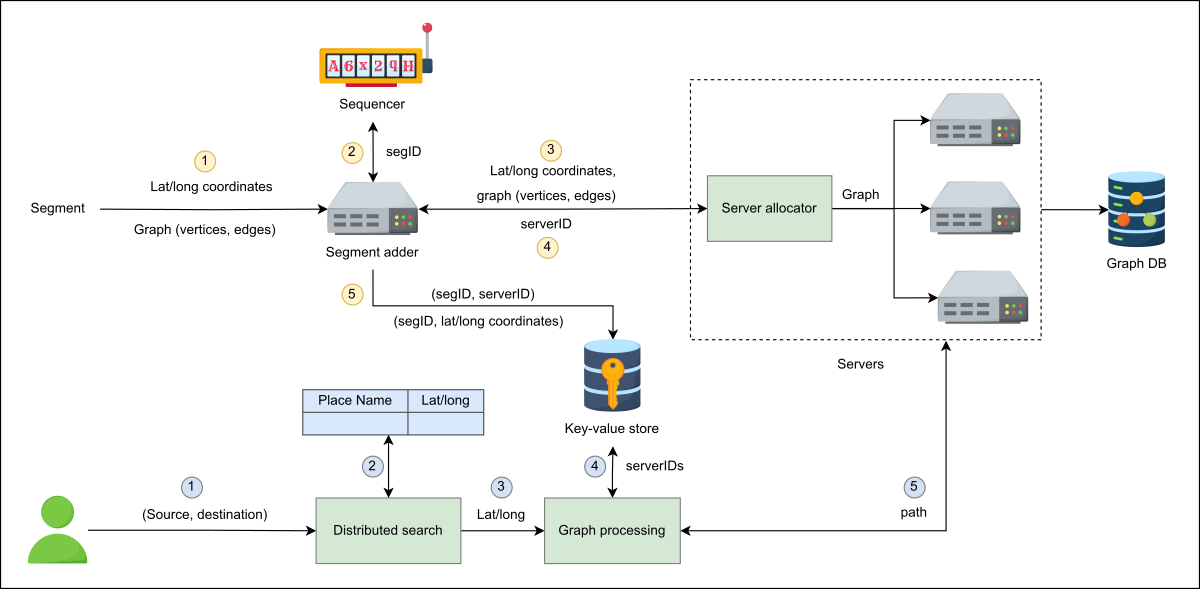
\includegraphics[width=0.5\textwidth]{Images/chapter_28/section_6026783136940032/5554400087375872.png}
 \caption{Workflow 1) Adding segments (in yellow), and workflow 2) Processing user requests (in blue)}
\end{figure}

\textbf{Add segment}

\begin{enumerate}
\item
\protect\phantomsection\label{D9PhzwmtZCagoXfrXNHMg}
Each segment has its latitude/longitude boundary coordinates and the graph of its road network.
\item
\protect\phantomsection\label{QeuMjxXmfHkLZVsKtGWB6}
The segment adder processes the request to add the segment along with the segment information. The segment adder assigns a unique ID to each segment using a unique ID generator system.
\item
\protect\phantomsection\label{ydruBZb6NI1MGT3rjchfP}
After assigning the ID to the segment, the segment adder forwards the segment information to the server allocator.
\item
\protect\phantomsection\label{Mw1p1F0TB5dMfR3My6Wil}
The server allocator assigns a server to the segment, hosts that segment graph on that server, and returns the \texttt{serverID} to the segment adder.
\item
\protect\phantomsection\label{fCql-34t_8GRiAN-R8XuX}
After the segment is assigned to the server, the segment adder stores the segment to server mapping in the key-value store. It helps in finding the appropriate servers to process user requests. It also stores each segment\textquotesingle s boundary latitude/longitude coordinates in a separate key-value object.
\end{enumerate}
\\
\textbf{Handle the user's request}

\begin{enumerate}
\item
\protect\phantomsection\label{aw_Grfc8lvVzg7Id4F6-k}
The user provides the source and the destination so that our service can find the path between them.
\item
\protect\phantomsection\label{Fx-feCJRD6DPLlQigmJeY}
The latitude and longitude of the source and the destination are determined through a distributed search.
\item
\protect\phantomsection\label{zYqanpNp0MEojLMBKTddV}
The latitude/longitude for the source and the destination are passed to the graph processing service that finds the segments in which the source and the destination latitude/longitude lie.
\item
\protect\phantomsection\label{0Rajun2_fmarCtklNJj_n}
After finding the segment IDs, the graph processing service finds the servers that are hosting these segments from the key-value store.
\item
\protect\phantomsection\label{twN6aEYqkiN9tuxGEeJn8}
The graph processing service connects to the relevant servers to find the shortest path between the source and the destination. If the source and the destination belong to the same segment, the graph processing service returns the shortest path by running the query only on a single segment. Otherwise , it will connect the segments from different servers, as we have seen in the previous lesson.
\end{enumerate}

\subsection{Improve estimations using live data}\label{41Ks7BgrV0YftbUZpXjaI}
\\
This section describes how we can improve the ETA estimation accuracy using live data. If we have a sequence of location data for different devices, we can find movement patterns and perform analytics to predict various factors that may influence a user's trip. Google Maps uses a combination of GPS, Wi-Fi, and cell towers to track users' locations. To collect this data, our maps system servers need to have a persistent connection with all the devices that have their location turned on. Below
, we discuss the tools, techniques, and components involved in the process of improving estimations using live data.

\begin{itemize}
\item
\protect\phantomsection\label{6h4W8n9e9jurkynpb94Sx}
\textbf{WebSocket} is a communication protocol that allows users and servers to have a two-way, interactive communication session. This helps in the real-time transfer of data between user and server.
\item
\protect\phantomsection\label{36idoOhGHkQgkVD6ejeuY}
The \textbf{load balancer} balances the connection load between different servers since there is a limit on the number of WebSocket connections per server. It connects some devices to server 1, some to server 2, and so on.
\end{itemize}

\begin{figure}[htbp]
 \centering
 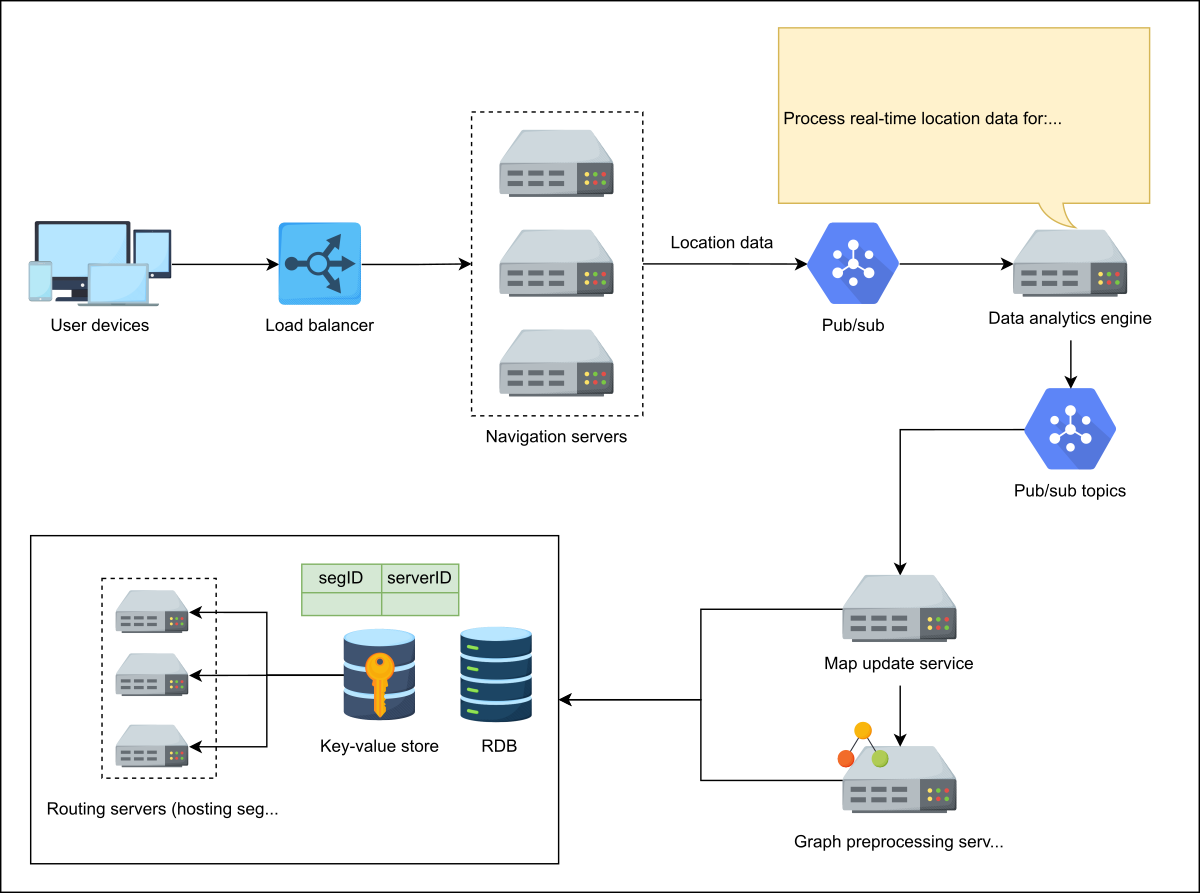
\includegraphics[width=0.5\textwidth]{Images/chapter_28/section_6026783136940032/5985168412508160.png}
 \caption{Performing analytics on the live location data to keep the map up-to-date and also improve ETA estimations}
\end{figure}

\begin{itemize}
\item
\protect\phantomsection\label{4xV4rQ56wKqhX5qOCXU2n}
A \textbf{pub-sub} system collects the location data streams (device, time, location) from all servers. The location data from pub-sub is read by a \textbf{data analytics engine} like Apache Spark. The data analytics engine uses data science techniques---such as machine learning, clustering, and so on---to measure and predict traffic on the roads, identify gatherings, hotspots, events, find out new roads, and so on. These analytics help our system improve ETAs.
\end{itemize}
\begin{quote}
\textbf{Note:} The amount of traffic, road conditions, and hotspots directly affect average travel speed, which ultimately affects users' ETAs.
\end{quote}
\begin{itemize}
\item
\protect\phantomsection\label{imWURPY3XCPgIimATcwRc}
The data analytics engine publishes the analytics data to a new \textbf{pub-sub topic}.
\item
\protect\phantomsection\label{aUDz1KiRDd_XCwmh8RD7y}
The \textbf{map update service} listens to the updates from the pub-sub topic for the analytics. It updates the segment graphs if there is a new road identified or if there is a change in the weight (average\ speed\ (traffic,\ road\ condition)) on the edges of the graph. Depending on the location, we know which segment the update belongs to. We find the \textbf{routing server} on which that segment is placed from the key-value store and update the graph on that server.
\end{itemize}

\begin{quote}
\textbf{Quiz:}
\textbf{Question 1:} Many traffic conditions are transitory (like stopping at a signal), so updating the graph very often wouldn't scale well because it requires excessive processing. What could be the solution to this problem?
\textbf{Answer:} To efficiently handle both normal and transitory traffic conditions in

Google Maps, the system maintains two sets of data for the routing graph's edge weights: one reflecting normal (historical or average) conditions, and another capturing transitory (temporary) events like signal stops or short-term congestion. This dual-data approach allows the system to avoid excessive processing and constant full-graph updates for every minor, fleeting change in traffic. When calculating routes,
the system overlays the transitory data on top of the normal conditions, applying only relevant and recent updates to routing decisions. As transitory events expire or clear up, their effects are automatically removed, ensuring that only significant and persistent changes impact the underlying graph, thus maintaining both accuracy and efficiency at scale.
\end{quote}

\begin{itemize}
\item
\protect\phantomsection\label{DL5cDB_L2J8ouOSYCu4Ck}
The \textbf{graph preprocessing service} recalculates the new paths on the updated segment graph. We've seen how the paths are updated continuously in the background based on the live data.
\end{itemize}
\\
We've learned how the segments work, how a user finds the location between two points, and how the ETA\textquotesingle s accuracy is improved by utilizing the live location data.

% End of section content